\chapter{Design of the Polymerase Evolution Model} % (fold)
\label{cha:design_of_the_polymerase_evolution_model}
This chapter provides a detailed description of the design of the model system used to investigate the question of the evolution of nucleotide polymerase directionality. The goal of this model is to have organisms containing either a $5'\to3'$ or a $3'\to5'$ nucleic acid polymerase compete with each other in order to see which of the strategies, if either, are evolutionarily dominant. In the model, evolutionary pressure is applied by the rate at which organisms can reproduce and the fidelity with which they duplicate their genomes. Evolutionary momentum is introduced through simple genetic mutation, which could be enabled or disabled on a per experiment basis. The model is also designed such that the influence of temperature on the outcome of this competition can be investigated.

\section*{Overview} % (fold)
\label{sec:overview}
In simplest terms, this model consists of a number of individual organisms in competition with each other. The model can be largely divided up into, and thought about most clearly as, four interacting components. These are the environment, the organisms, the genomes, and the polymerases. The relationship between these components begins with the environment. Each run of the simulation involves exactly one environment. An environment may contain many organisms, up to a predefined carrying capacity, and at the beginning of a simulation run the environment is pre-populated organisms according to a set rules.

Each organism contains one genome. At the start of an organisms ``life'', it uses its genome to create a polymerase. The polymerase replicates either $5'\to3'$ or $3'\to5'$ and may not change direction. The polymerase then replicates the genome at a predetermined rate and with a random chance of introducing errors (mutations). When the polymerase is finished duplicating the genome, the organism will attempt to divide by binary fission using the newly created genome. If it is successful in doing so, then the new organism is added to the environment and begins a fresh life cycle while the original organism resets itself and also begins a fresh cycle.

A number of generalizations and assumptions have been made in order to render the problem being investigated tractable, but a consistent effort has been made to remain as true to life as possible. The motivation behind this is that, while the exact values generated by this model may not be precisely those that would be observed in the laboratory, the trends observed should hold true when transferred to the bench. For each piece decisions have been made regarding which aspects of the component are explored in depth, and which aspects are neglected, with an eye to the larger goal of investigating the role of polymerase directionality. Following is a detailed look at each component in turn.
% section overview (end)

\section*{Environment} % (fold)
\label{sec:environment}
At the start of a simulation run, the environment for that run is initialized with a starting population of organisms. To create this starting population, a set of organisms with their genome length, polymerase rate, and polymerase directionality specified is divided according each organism's designated frequency in the starting population. The starting population size can be any number up to the specified maximum population of the environment.

A key defining feature of this model is that the environment is constrained in some ways, but not in others. Specifically, the number of organisms that can simultaneously co-exist has a hard numerical limit; a carrying capacity. On the other hand, the amount of available energy, the quantity of activated nucleotide triphosphates, and the other raw materials required for forming a cell are all considered unlimited. In reality, the carrying capacity is a generalization that could correspond to physical space limits, but it could just as easily correspond to the aggregate limitations on the other resources not explicitly modeled.

The choice of limitation based on carrying capacity was driven by two factors. The first relates to the fact that selection during an exponential growth phase could potentially operate differently than during stationary phase growth. By placing an upper limit on the size of a population, it is possible to investigate selection during both growth phases. Second, while attempting to explicitly model all of the various resource and space constraints that might ultimately limit growth might yield a more complete model, it would also significantly increase the complexity of the model without adding much insight into the question at hand. Finally, numerically or density limited growth is a common observation across a wide range of living creatures from single cells to large populations of complex animals\cite{Ferenci:1999p703}.

In order to model density dependent growth inhibition as the number of organisms approaches the carrying capacity, a random death probability is introduced to the environment. In keeping with observations that the pressure of density dependent inhibition is greater as the population of an environment approaches the carrying capacity, the death probability is calculated with an inverse function of the remaining capacity\[
	P_{death} = \frac{1}{(N-n)+1}
\]where $N$ is the carrying capacity, $n$ is the number of organisms currently in the environment, and $1$ is added so that the probability of at least one organism being culled from the environment when the carrying capacity is reached is $P_{death}=1$.

The model iterates its environment in a stepwise fashion. During each step, each of the organisms contained within the environment is allowed to carry out one time-step of its life cycle, followed by a population culling. Culling is carried out by calculating the death probability as above, and then randomly applying that probability to the environment to decide if an organism should be removed. If the decision is made to remove an organism, one is chosen from the environment randomly, removed, and the death probability is recalculated and reapplied. This process will repeat until the decision is made not to remove an organism. In this way, the number of organisms removed at each time step follows a Poisson distribution with an expectation value of $P_{death}$.
% section environment (end)

\section*{Organism} % (fold)
\label{sec:organism}
Organisms are created and added to the environment either at the start of a simulation run, as part of the starting population, or during the simulation run as the result of binary fission of an existing organism. If the organism is created at the start of the simulation then its genome and polymerase properties are determined by the values used to seed the population. Each of these seed organisms is generated with a random amount of its genome already synthesized, to avoid synchronization artifacts that arise if all organisms start polymerizing from zero at the start of the simulation.

If the organism is created during a simulation run, then its properties are derived from those of its parent, with the possibility of introduced variation. This variation is embodied by, and in the model determined by, the genome contained within the organism. Each organism contains exactly one genome and one polymerase. Having only one polymerase is a simplification, but it is justified by considering this one polymerase as an exemplar of all the polymerase enzymes that would be found in a real organism.

Each organism is modeled as a state machine. The two states in which an organism can exist are: \emph{Polymerizing} or \emph{Duplicating}. At creation, each organism starts in the \emph{Polymerizing} state. When an organism is in the \emph{Polymerizing} state, each simulation time-step is used to allow the organism's polymerase to add nucleotides to the genome copy being constructed. At the end of each time-step, the polymerase is queried as to whether or not it is finished with constructing the nascent genome. If it is, then the organism shifts to the \emph{Duplicating} state. Otherwise, it remains in the \emph{Polymerizing} state.

When an organism reaches the \emph{Duplicating} state, a check is performed to determine if the genome copy constructed by the polymerase is viable. This is a simple sanity check to ensure that the synthesized genome is of the correct length. If the genome copy is not viable, then it is discarded and the organism returns to the \emph{Polymerizing} state to create a new genome copy. If the genome is viable, the next determination that must be made is whether or not there is available capacity in the environment for a new organism.

If the number of organisms in the environment is not at the environment's carrying capacity at the start of a simulation time step, then an organism in the \emph{Duplicating} state can proceed to create a new organism. The thus created organism containing the newly synthesized genome is inserted into the environment. In this case, the parent organism will return to the \emph{Polymerizing} state to begin construction of yet another new genome. If, instead, the environment is at capacity at the start of a simulation time step, then any organism in the \emph{Duplicating} state will remain unchanged, in the \emph{Duplicating} state. It will next attempt to add a new organism with the synthesized genome during the next environment step.
% section organism (end)

\section*{Genome} % (fold)
\label{sec:genome}
Genomes are created before the organism in which they are contained. In the case of a running simulation, the new genome is created by the parent organism before binary fission. For the starting population of organisms used to seed a simulation, the genomes are created ahead of time with predefined properties and a random amount of replication already completed. The model genomes perform three important functions for the simulation: they generate polymerases with properties defined by the genome, they track the progress of the organism's polymerase during polymerization, and they return a copy of themselves once polymerization has completed.

Each genome codes for either a $5'\to3'$ polymerase or a $3'\to5'$ polymerase, and this will not change through subsequent generations. There is the possibility that this is not perfectly reflective of how early organisms may have functioned, as it is conceivable that, through acquired mutations, a genome which coded for a $3'\to5'$ polymerase may evolve in subsequent generations into a genome that codes for a $5'\to3'$. Were this to occur, it would either have to be through a gradual mechanism or a small mutation affecting global properties of the polymerase. A gradual mechanism would be one where the forward or reverse speed of the polymerase is reduced to nearly zero, and then eventually the directionality flipped. It is safe to eliminate this possibility in the model, as such a transition would require the survival of an organism with an especially slow polymerase. As a consequence of the starting assumption that polymerase speed is the primary determining factor in the speed of replication, such organisms would be quickly out-competed in the simulation.

The alternative mechanism of a small mutation leading to a global change can also be neglected for two reasons. First, if such a mutation were possible, the fidelity of communicating polymerase directionality from one generation to the next would be diminished. This would imply that selecting against a $3'\to5'$ polymerase would effectively be impossible, as such polymerases could appear at almost any time. This would also narrow the window of possible founder populations were the alternate founder effect hypothesis considered. In the case that polymerase directionality were trivially reversible, the hypothetical founder population would not only have to be homogenous in their polymerase directionality, but they would also have to have a unique restriction on the directionality reversing randomly. This also highlights the second reason that the possibility of such a mutation need not be considered: if such mutations were possible, it would be expected that they could be observed today. Certainly, it is possible that such a mutation might have existed in the past but have subsequently been locked out of the population of current polymerase sequences, but this seems unlikely. Nucleotide polymerases are wildly variable in their sequence and structure throughout all forms of life, and yet none exhibit reversed directionality.

When a genome is asked by its organism to create a polymerase, it will imbue the polymerase with a fixed polymerase rate in addition to a fixed directionality. The precise value the polymerase speed will take is determined when the genome is created from its parent (or from predefined values at the beginning of a simulation). Once the polymerase has been generated and polymerization begun, the polymerase will inform the genome during each simulation time-step how many nucleotides have been added to the copy being created, and how many of those are erroneous base pairs. The genome keeps track of this information for later reporting and calculations.

When a genome copy is constructed, the genome can then provide that copy to a new organism, but in doing so it must determine the properties of this new genome. As mentioned above, the directionality is inherited exactly. The polymerase speed coded for by the copy genome is determined in a two step calculation based on the number of errors (mutations) introduced. First, the variance from the parent genome's encoded polymerase rate is calculated by taking\[
	\Delta = \frac{r_{max} - r_{min}}{2}*\frac{M}{M_{max}}
\]
where $r_{max}$ and $r_{min}$ are the maximum and minimum possible rates, respectively, $M$ is the number of errors made during replication, taken as a fraction of total genome length, and $M_{max}$ is the maximum tolerated fraction of errors, which was set at $\frac{1}{3}$. The maximum tolerated fraction of errors is the threshold above which it can be assumed that the inherited traits of the polymerase are, essentially, selected at random. The maximum and minimum rates were chosen as 1 and 10 nucleotides added per simulation time-step to reflect the roughly 10-fold range of empirically observed polymerase rates.

The logic behind this metric is that more mutations will, on average, lead to greater alteration of enzyme function. Certainly there are individual mutations that could, on their own, have a large effect on polymerase rate, but averaged over many polymerases and many possible mutations, this general trend should hold. Once the variance is determined, it must be applied to the parent genome's encoded polymerase rate in such a way that the child's genome does not code for an invalid polymerase. So, if the variance would generate a polymerase rate above the maximum, then it is subtracted from the parent rate, and vice versa. If the variance would not result in an invalid rate as a consequence of either addition or subtraction, then it is applied to the parent rate with an equal probability of either outcome.
% section genome (end)

\section*{Polymerase} % (fold)
\label{sec:polymerase}
The single most significant component of the model is the model nucleotide polymerase itself. The other three components described above serve primarily to ensure that selection and descent with modification will occur, but it is the polymerase which embodies the trait that is ultimately being selected for or against: the polymerase's directionality. As with the genomes, the directionality and rate of a polymerase does not change subsequent to its creation. These properties are determined by the genome from which the polymerase is generated. The polymerases only have one function during a simulation: to add nucleotides to a growing genome copy. How this occurs depends on the polymerase directionality and the temperature of the simulation.

When an organism in the \emph{Polymerizing} state carries out one step of simulation time, the polymerase will add nucleotides to the genome being synthesized. The polymerase does this by running through a loop with a maximum number of iterations determined by its rate. So, for example, a polymerase with a rate of 7 can carry out its nucleotide addition loop a maximum of 7 times for each 1 simulation time step. During each loop, two determinations must be made. First, the polymerase must determine whether the nucleotide about to be added is activated, and second it must determine whether a properly base-paired nucleotide is being added, or whether the nucleotide being added will generate a replication error.

The reason that the polymerase must determine whether or not the nucleotide being added is activated is due to a consequence of chemistry. All known nucleotide polymerases in nature use, as their substrate, nucleotide triphosphates. They use the energy released by cleaving the bond between the $\alpha$ and $\beta$ phosphates attached to their $5'$ carbon to drive the polymerase reaction forward. However, this bond can be cleaved through spontaneous hydrolysis by water. The equilibrium between active and inactive nucleotides can be described by a Boltzmann distribution:\[
	K = e^{-\frac{\Delta G^0}{RT}}
\]
where $\Delta G^0$ is the standard free energy of the hydrolysis reaction. To simplify the simulation calculations, the entire $\frac{\Delta G^0}{RT}$ term is expressed as a generic simulation temperature $\frac{1}{t}$.

Where this process of inactivation becomes important is in how it will differentially affect a $5'\to3'$ polymerase vs a $3'\to5'$ polymerase. In the $5'\to3'$ case, the one that is observed in all known forms of life, the triphosphate is attached to the incoming nucleotide about to be added to the chain. If this incoming nucleotide becomes inactive before the polymerase has a chance to join it to the growing nucleic acid polymer, then this represents a wasted addition step. That is, if a polymerase with a rate of 7 has one of its nucleotides become inactive before phosphodiester bond formation, then it will only add 6 nucleotides during this simulation time-step.

On the other hand, in the case of a hypothetical $3'\to5'$ polymerase, the triphosphate group would be attached to the $5'$ carbon of the nascent nucleic acid polymer. If this triphosphate is cleaved during an addition step, the polymerase will not be able to compensate by drawing in a new nucleotide from the pool of available nucleotides. Rather, the polymerization process will necessarily halt while the terminal end of the growing chain is reactivated. In the simulation, that process is modeled by terminating the polymerase's addition of new nucleotides when an inactivation event occurs. That is, if a $3'\to5'$ polymerase with a rate of 7 experiences inactivation during the addition of the 3rd nucleotide in this time step, then only 2 new nucleotides will be added to the growing genome during this particular step.

Furthermore, whereas a $5'\to3'$ polymerase will be constantly drawing in new, activated nucleotides from the pool of all available nucleotides, a $3'\to5'$ polymerase depends on the nascent chain remaining activated. The consequence of this is that the probability of a $5'\to3'$ polymerase experiencing a deactivation event depends only on the free energy of the reaction and temperature, irrespective of polymerase rate. Alternatively, a $3'\to5'$ polymerase runs a greater risk of the triphosphate on the nascent chain becoming deactivated the longer it waits before adding a new nucleotide. So, for the reverse polymerases, the distribution was adjusted by a factor determined by the polymerase rate:\[
	K = e^{-\frac{1}{t}}*(r_{max} - r + 1)
\] where $r_{max}$ is the maximum polymerase rate and $r$ is the rate of the polymerase doing the addition. This extra factor accounts for the fact that a slower reverse polymerase will give each terminal phosphate group on the growing chain a longer period of time before addition of the next nucleotide monomer during which a spontaneous hydrolysis might occur.

Finally, each time a new nucleotide is added by a polymerase, there is a risk that the nucleotide will be of the wrong sort. The primary driving force discriminating properly base-paired nucleotides from improperly paired nucleotides is the formation of hydrogen bonds between the incoming nucleotide and the corresponding nitrogenous base of the template nucleic acid. The hydrogen bond interaction that allows discrimination between Watson-Crick base-pairing and a variety of mismatches was modeled using the same sort of Boltzmann distribution as used for the spontaneous hydrolysis condition. However, since the $\Delta\Delta G_0$ of a correct versus incorrect base pairing is twice that of the spontaneous hydrolysis reaction\cite{Petruska:1988p721,Bagshaw:1973p728}, the hydrogen bond portion of the erroneous inclusion calculation is made using the formula:\[
	P_{H-bond} = e^{-\frac{2}{t}}
\]
where $t$ is the simulation temperature.

Recently, research has indicated that hydrogen bond formation is not sufficient to completely explain the fidelity of correct pair formation by nucleotide polymerases. It has been suggested that polymerases also take advantage of geometric differences between proper and improper pair formation to improve their ability to discriminate correct versus incorrect base pairing. Prior studies have revealed a relatively complex link between polymerase rate and error rate for nucleotide polymerases\cite{Cady:2009p718}. The essence of this link is that there is an additional geometric constraint on erroneous nucleotide inclusions and that, in order to polymerize faster, polymerases must relax this constraint.

In the model, this additional factor is treated as a simple flow problem. If a polymerase is roughly represented as a cylindrical tube, the narrower the tube is the greater will be its ability to reject geometrically unfavorable nucleotide pair configurations. However, the rate of the polymerase will also be affected by the radius of the tube (see figure~\ref{fig:schematic} for an illustration of this concept). If rate is taken as the flux of nucleic acid through the tube, then we end up with a simple square root relationship between the ability of the polymerase to reject based on geometry and the number of nucleotides it can add in one simulation time-step. Specifically\[
	\Gamma = \sqrt{r}
\]
describes the geometric discrimination and\[
	P_{error} = K * \Gamma
\]
is the probability of making a mistake during each nucleotide addition event, calculated as the product of the temperature dependent Boltzmann distribution, $K$, and the geometric discrimination function, $\Gamma$. Alternatively, in order to investigate the effect of mutation on evolution, $P_{error}$ could be artificially set to 0 at the start of a simulation run.

\begin{figure}[ht]
	\centering
		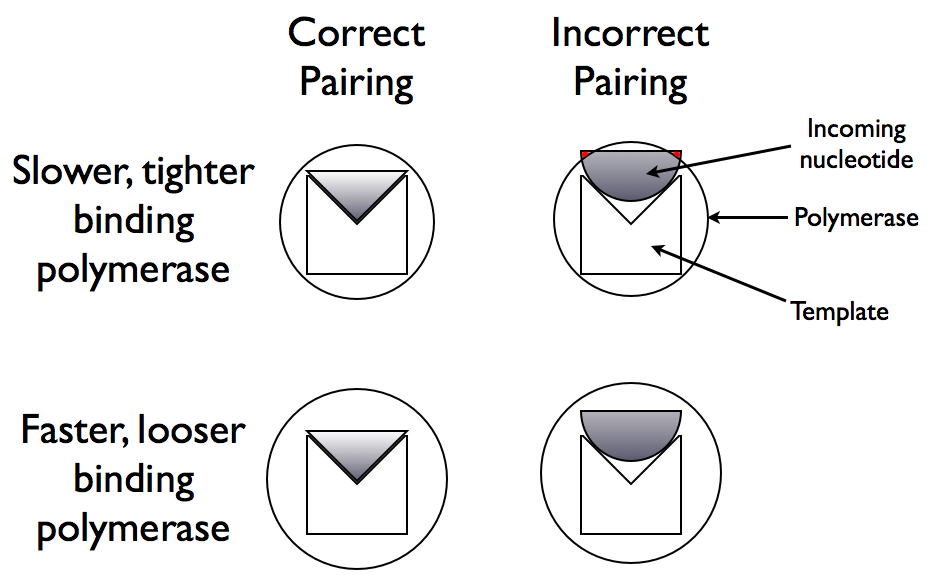
\includegraphics[width=\textwidth]{schematic}
	\caption{\textbf{A schematic diagram of geometry based polymerase discrimination.} The simplistic model of geometry based discrimination, and its relationship to polymerase rate, assumes that a tighter binding polymerase will be better able to exclude incorrect nucleotides based on shape. However, being tighter binding will restrict the rate at which the polymerase can translocate along the nucleic acid.}
	\label{fig:schematic}
\end{figure}

% section polymerase (end)
% chapter design_of_the_polymerase_evolution_model (end)